\chapter{Concept Development}
\label{chap:concept-development}

This chapter converts the findings from the literature review in Chapter~\ref{chap:state-of-research} and the requirements defined in Chapter~\ref{chap:requirements-analysis} into concrete structural decisions for the AI-based classification system.

This section of the thesis explains the background behind selecting the CNN architectures, the processing pipeline, the training strategy, the hyper-parameter selection, the evaluation setup, and the Grad-CAM analysis.

These decisions establish the basis for the implementation described in the next chapter which is Chapter~\ref{chap:implementation}.

\section{Selection of CNN Architectures}

Three CNN architectures were selected for this thesis: ResNet50, ResNet18, and MobileNet. The selection was based on two main factors from the literature review: classification performance and computational efficiency.

Since classification performance is an important objective of this work, ResNet50 and ResNet18 were selected as the main residual architectures. As discussed in Section~\ref{sec:cnn_classification}, Rajaraman et al. \cite{{Rajaraman2018} evaluated several CNN architectures for malaria cell classification using patient-level cross-validation. ResNet50 achieved high classification performance compared with the other tested architectures. ResNet18 was added as a smaller ResNet variant to investigate whether a less complex residual network can achieve comparable classification performance.

MobileNet was selected as the lightweight architecture for the intended system. As discussed in Section~\ref{sec:lightweight_networks}, lightweight CNN architectures are useful when computational resources are limited, which is relevant to this project. MobileNet reduces computational effort by using depth-wise separable convolutions and is therefore suitable for comparing classification performance with a more efficient network design. This is important for the intended PC-based diagnostic system and also for possible future deployment where computational resources are limited.

The three architectures were therefore selected to represent two different goals. ResNet50 and ResNet18 focus more on classification performance, while MobileNet represents the lightweight side of the comparison. This addresses the two aspects of the research gap identified in Section~\ref{sec:research_gap}: achieving strong classification performance while also considering computational efficiency.

\section{Processing Pipeline}

The processing pipeline describes how a thick blood smear image is transformed from the original input into a classification result. It represents the AI-related part of the overall system introduced in Chapter~\ref{chap:system-overview}.

The overall processing pipeline is shown in Figure~\ref{fig:processing_pipeline}.

\begin{figure}[htbp]
    \centering
    \fbox{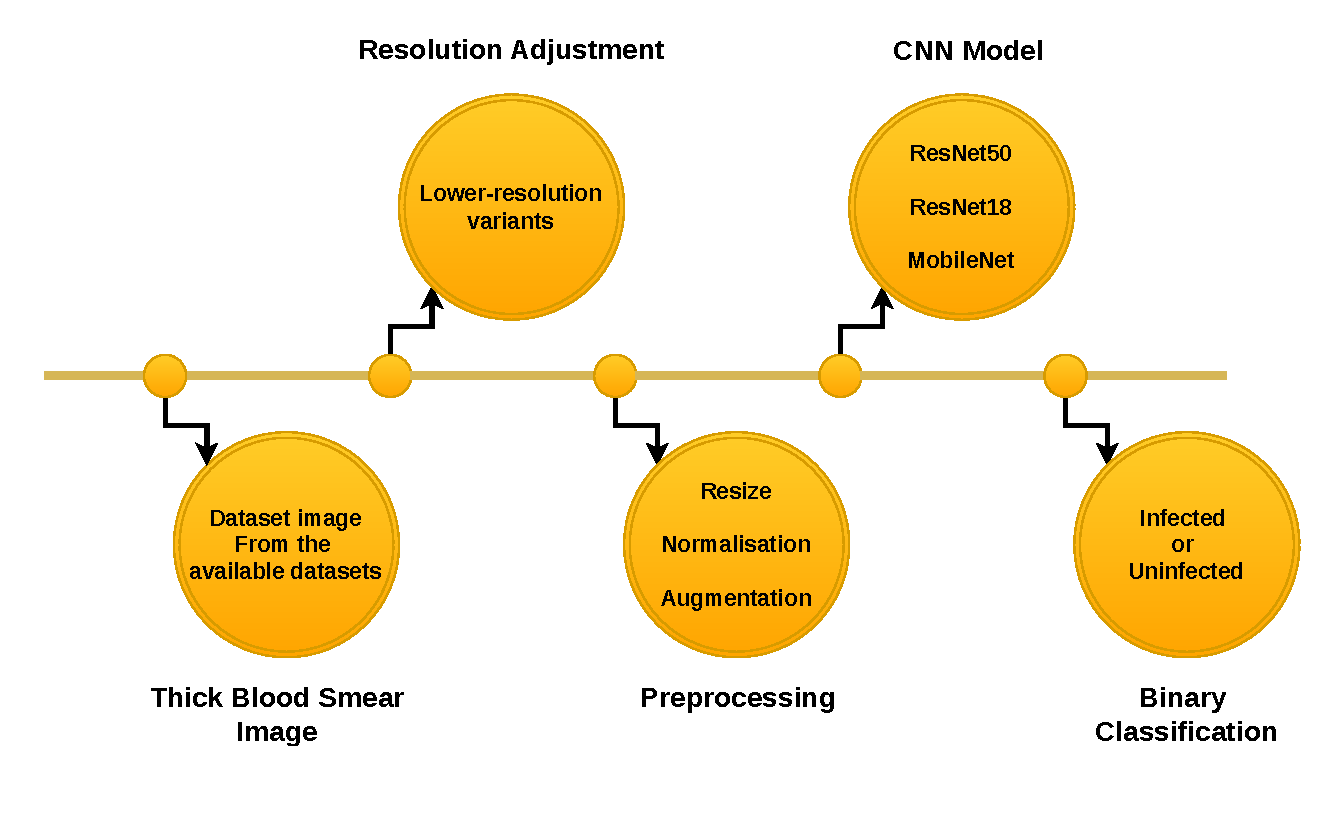
\includegraphics[width=0.9\textwidth]{Processing_Pipeline.pdf}}
    \caption{Processing pipeline of the AI-based malaria classification system.}
    \label{fig:processing_pipeline}
\end{figure}

\FloatBarrier

A complete thick blood smear image is used as an input for classification, without detecting parasite regions or identifying parasite types. The goal is to classify each image as either infected or uninfected, which is the main goal of this thesis. This differs from many of the reviewed approaches in chapter~\ref{chap:state-of-research}, which first extract parasite regions or cell-level areas before classification.

Before the image is passed to the CNN model, preprocessing is applied. This includes normalisation and resizing to the input size required by the selected architecture. During training, data augmentation is also used.

For the resolution experiments, the same source images are processed at different resolution levels in separate runs. The image is first reduced to the selected lower resolution and is then resized to the input size expected by the model. This makes it possible to compare how the same architecture behaves under different image resolutions.

The preprocessed image is then passed through one of the selected CNN architectures: ResNet50, ResNet18, or MobileNet. The model produces a binary classification result predicting whether the image is infected or uninfected.

\section{Training Strategy}
\label{sec:training_strategy}

The selected CNN models are trained using transfer learning. To save time and computing power, pretrained ImageNet weights are used as the starting point for the models. The models are then fine-tuned using the malaria thick blood smear images. This approach makes it possible for the networks to start from already learned image features and adapt them to the task of malaria classification.

The final classification layer is adapted to two output classes: infected and uninfected. Cross-entropy loss, explained in Section~\ref{sec:deep_learning_fundamentals}, is used during the training to show how wrong the model’s prediction is compared with the correct class. Adam is then used as the optimiser for updating the model parameters during training. The same training strategy is applied to ResNet50, ResNet18, and MobileNet in order to keep the comparison between the architectures more fair.

To support model generalisation, data augmentation is applied only to the training images. The augmentation includes horizontal and vertical flipping as well as small image rotations. The goal is to increase the variation of the training data and reduce the risk of overfitting. The validation images are not augmented.

During training, the validation accuracy is calculated after each epoch. Each time a higher validation accuracy is reached, the corresponding checkpoint is saved. If the same validation accuracy is reached again, the previously saved checkpoint is kept. The checkpoint with the highest validation accuracy is later used for the final test evaluation.

\section{Hyperparameter Selection}

The hyperparameters were selected based on the available hardware. Since the training was performed on a MacBook Pro with an M2 chip and 8 GB of memory, moderate settings were chosen to keep the training stable and manageable.

The same main hyperparameters were used initially for ResNet50, ResNet18, and MobileNet. A learning rate of 0.0001, which is suitable for fine-tuning pretrained models, was used together with the Adam optimiser. The batch size was set to 8, and each model was trained for 15 epochs. The pretrained networks were fine-tuned as complete models rather than keeping the earlier layers frozen.

Using the same training parameters for all three architectures makes the comparison more reliable by reducing the effect of different hyperparameter settings on the results. It is also planned that, if one of the lightweight models shows very low performance, an additional optimisation may be carried out. This approach was also discussed within the project team and was considered suitable for a fair comparison of the selected architectures.

After each epoch, the validation accuracy was calculated, and the checkpoint with the highest validation accuracy was saved for later evaluation.

\begin{table}[htbp]
\centering
\caption{Main hyperparameters used for training.}
\label{tab:hyperparameters}
\begin{tabularx}{\textwidth}{|p{5cm}|X|}
\hline
\textbf{Hyperparameter} & \textbf{Selected value} \\
\hline
Learning rate & 0.0001 \\
\hline
Batch size & 8 \\
\hline
Number of epochs & 15 \\
\hline
Optimizer & Adam \\
\hline
Weight initialization & pretrained on ImageNet\\
\hline
Fine-tuning & Complete network \\
\hline
Model selection & Highest validation accuracy \\
\hline
\end{tabularx}
\end{table}

\FloatBarrier

\section{Evaluation Setup}

The evaluation is constructed to compare the selected CNN architectures for this work under the same conditions and to investigate how reduced image resolution affects the classification performance.

The high-resolution baseline uses an image size of \(224 \times 224\) pixels, which corresponds to the standard input size used by the pretrained ResNet and MobileNet models. For the reduced resolution experiments, the same source images are reduced to lower resolutions (LR1/LR2/LR3) and then resized back to \(224 \times 224\) pixels before being given to the CNN model. In this way, the input size of the network stays unchanged while the amount of image detail is reduced. The lowest tested resolution is \(56 \times 56\) pixels and represents the extreme low-resolution case.

The dataset is divided into training, validation, and test sets using a standards patient-based split of 70\%, 15\%, and 15\%. All images belonging to the same patient remain in the same subset. This avoids using images from the same patient for both training and evaluation.

The classification performance is evaluated using accuracy, sensitivity, specificity, precision, F1-score, and ROC-AUC. These metrics were already explained in Section~\ref{sec:deep_learning_fundamentals}. Using several metrics makes it possible to evaluate the overall classification accuracy as well as the behaviour of the models for infected and uninfected images.

The experiments are carried out in several steps. First, a high-resolution baseline is established. The influence of reduced image resolution is then investigated using lower-resolution runs of the same images. At the end, the selected CNN architectures are compared under the defined evaluation conditions. This approach reduces the number of unnecessary training runs while allowing the influence of image resolution to be investigated.

\captionsetup[table]{skip=2pt}
\begin{table}[htbp]
\centering
\caption{Resolution levels used in the evaluation.}
\label{tab:resolution_levels}
\begin{tabularx}{\textwidth}{|p{3cm}|X|}
\hline
\textbf{Resolution level} & \textbf{Image size} \\
\hline
HR & 224$\times$224 pixels \\
\hline
LR1 & 160$\times$160 pixels \\
\hline
LR2 & 112$\times$112 pixels \\
\hline
LR3 & 56$\times$56 pixels \\
\hline
\end{tabularx}
\end{table}

\FloatBarrier

\section{Grad-CAM Analysis}

During the test phase, Grad-CAM is used to understand the behaviour of models that show weak performance. As discussed in Section~\ref{sec:explainability}, Grad-CAM generates a heatmap that highlights the image regions that have the strongest influence on a prediction.

The analysis is therefore focused on underperforming cases, for example models or resolution settings with lower classification performance. The goal here is to investigate whether the model still focuses on meaningful regions inside the microscopic image, for example areas containing parasites, or whether the prediction is influenced by unrelated areas such as the background or image edges.

Grad-CAM is also applied to some selected true-positive, true-negative, false-positive, and false-negative predictions. This makes it possible to compare successful and incorrect classifications and to better understand how the model behaves in different prediction cases.

The Grad-CAM analysis is used as a supporting method together with the evaluation metrics. This helps to identify reasons for unusual model behaviour that cannot be explained by accuracy, sensitivity, specificity, or F1-score alone. The generated heatmaps are presented and discussed in the evaluation chapter.